% =====================================================================
% Skeleton F — 4 Phase Horizontal + Multi Vertical Sub-elements per Phase
% =====================================================================
% USAGE: Adapted from a GOLD STANDARD figure (Privacy-Preserving MPC
% Protocol). Sub-agent: copy ENTIRE file as figure.tex, change content.
%
% ⚙ LAYOUT = BY-CONSTRUCTION (positioning + fit + node anchors): the 4
%   phase columns are chained off named pitch macros, sub-boxes stack with
%   below=of, zone backgrounds use fit, cross-phase arrows ride node
%   anchors. Change content / restack sub-boxes and the rest REFLOWS.
%   ⚠ The "uniform y=16.8 / y=16.5 / y=6.0" chip+zone numbers and the CRS
%   y=8.25 / Security y=6.2 below are ORIGINAL design intent — alignment is
%   now uniform BY CONSTRUCTION (chips anchored to each zone .north; zones
%   share one height; sub-boxes stacked by positioning), so manual y
%   bookkeeping no longer applies. SEMANTIC constraints (renaming, ≤6-char
%   bar labels, shares-below-box, keep-hero-right-empty, perf-box sizing)
%   STILL HOLD.
%
% LAYOUT MODEL:
%   ┌───────────┬───────────┬───────────┬───────────┐
%   │ Phase 1   │ Phase 2   │ Phase 3   │ Phase 4   │
%   │  Setup    │  Encrypt  │  Compute  │  Output   │
%   │ ┌───────┐ │ ┌───────┐ │ ┌───────┐ │ ┌───────┐ │
%   │ │ Sub-1 │ │ │Party A│ │ │ Hero  │ │ │ Recv  │ │
%   │ │ Sub-2 │ │ │Party B│ │ │ Multi │ │ │  ZK   │ │
%   │ │ Sub-3 │ │ │Party C│ │ │ layer │ │ │  Perf │ │
%   │ └───────┘ │ └───────┘ │ └───────┘ │ └───────┘ │
%   └───────────┴───────────┴───────────┴───────────┘
%   Each phase = container with 3+ vertical sub-elements inside.
%
% WHEN TO USE: Multi-party protocols (MPC, threshold sig), staged
% systems with internal sub-elements per stage (vs single hero per stage).
%
% CONTAINS: 4 phase containers + Phase 1 (3 setup sub-blocks) + Phase 2
% (3 parallel parties) + Phase 3 (Garbled Circuit + OT + Eval hero) +
% Phase 4 (Output Recovery + ZK Verification + Performance bar).
%
% CONSTRAINTS — DO NOT VIOLATE (each one fixed a real bug):
%
%   [RENAMING]
%   - 4 phase names (Setup/Encrypt/Compute/Output) — RENAME to topic stages.
%   - 3 parties in Phase 2 (A/B/C) — RENAME.
%   - Phase 3 hero (Garbled Circuit / OT / Eval) — RENAME.
%   - Phase 4 sub-elements (Output Recovery / ZK Verify / Performance) — RENAME.
%   - Performance bar labels (Setup/Online/Verify/Total) MUST be ≤ 6 chars
%     each — longer labels truncate inside the 3.6cm-wide chart.
%
%   [PHASE CHIPS + ZONES — uniform appearance is required]
%   - All 4 phase chip labels positioned at uniform y=16.8 with the same
%     anchor convention. Inconsistent anchors look ragged.
%   - All 4 zone tops uniform y=16.5; all 4 zone bottoms uniform y=6.0.
%
%   [PARTY BOXES (Phase 2) — shares matrix placement]
%   - The small "shares" matrix for each party goes BELOW the party box
%     (y below ybase), NOT inside the box — it overlaps the centered
%     formula text inside the box otherwise.
%
%   [PHASE 3 HERO — keep right side clean]
%   - Do NOT add a "Gate count" or any side chart to the right of the
%     Eval formula box. A previous version had this and it always
%     overlapped the formula. The right region must stay empty.
%
%   [PHASE 4 PERFORMANCE BOX — strict sizing]
%   - Box width = 3.6cm (NOT 4.0cm). It must leave margin against the
%     4.0cm-wide Phase 4 zone, or it visually hugs the zone edge.
%   - x-axis arrow tip x ≤ 3.3 (in local Performance coords). x=3.6
%     overflows the 3.6cm box and the arrow pokes out.
%
%   [CRS / SECURITY NOTES — vertical stacking]
%   - CRS Setup at y=8.25; Security note at y=6.2 (NOT y=7.6 — that
%     overlapped CRS in a previous version).
% =====================================================================

\documentclass[tikz,border=25pt]{standalone}
\usepackage{tikz}
\usepackage[fontset=none]{ctex}
\setCJKmainfont{PingFang SC}
\setCJKsansfont{PingFang SC}
\usepackage{amsmath,amssymb}
\usetikzlibrary{shapes, arrows.meta, positioning, fit, backgrounds, calc, shadows, shapes.geometric}

% ===== 学术配色（新默认） =====
\definecolor{acaBlueLine}{HTML}{6080B0}      \definecolor{acaBlueFill}{HTML}{DBEAFE}
\definecolor{acaGreenLine}{HTML}{30A060}     \definecolor{acaGreenFill}{HTML}{A0D0A0}
\definecolor{acaOrangeLine}{HTML}{D06020}    \definecolor{acaOrangeFill}{HTML}{FFE6CC}
\definecolor{acaPurpleLine}{HTML}{6020D0}    \definecolor{acaPurpleFill}{HTML}{E1D5E7}
\definecolor{acaRedLine}{HTML}{B05050}       \definecolor{acaRedFill}{HTML}{F8CECC}
\definecolor{acaGreyLine}{HTML}{666666}      \definecolor{acaGreyFill}{HTML}{F5F5F5}
\definecolor{acaGoldLine}{HTML}{D09000}      \definecolor{acaGoldFill}{HTML}{F8F8E0}
\definecolor{acaTealLine}{HTML}{009060}      \definecolor{acaTealFill}{HTML}{D1FAE5}
\definecolor{acaCyanLine}{HTML}{00B0D0}      \definecolor{acaCyanFill}{HTML}{E0F7FA}
\definecolor{acaPinkLine}{HTML}{D06090}      \definecolor{acaPinkFill}{HTML}{FCE4EC}
\definecolor{acaYellowLine}{HTML}{E0C060}    \definecolor{acaYellowFill}{HTML}{FFF8E1}
\definecolor{acaLimeLine}{HTML}{80B060}      \definecolor{acaLimeFill}{HTML}{E8F5E9}
% Zone 背景
\definecolor{zoneBlueBg}{HTML}{E0E0F8}
\definecolor{zoneGreenBg}{HTML}{ECFDF5}
\definecolor{zonePurpleBg}{HTML}{F5F3FF}
\definecolor{zoneRedBg}{HTML}{F8E0E0}
\definecolor{zoneYellowBg}{HTML}{F8F0C0}
% 热力图
\definecolor{heatDeep}{HTML}{401090}
\definecolor{heatDark}{HTML}{6020D0}
\definecolor{heatMid}{HTML}{8B5CF6}
\definecolor{heatLight}{HTML}{C4B5FD}
\definecolor{heatBg}{HTML}{EDE9FE}
% 数据图表
\definecolor{barBlue}{HTML}{3080C0}
\definecolor{barGreen}{HTML}{30A060}
\definecolor{barOrange}{HTML}{D06020}
\definecolor{barRed}{HTML}{E03030}

\pgfdeclarelayer{background}
\pgfsetlayers{background,main}

% ---- single source of truth for layout rhythm ----
% Column pitches are centre-to-centre. They differ because the four phases
% have different widths (Phase 3 is the wide hero); each pitch is defined
% ONCE here and the column centres are chained off them below.
\def\gapAB{6cm}    % Phase 1 -> Phase 2
\def\gapBC{6.5cm}  % Phase 2 -> Phase 3 (wider: hero column)
\def\gapCD{5.5cm}  % Phase 3 -> Phase 4
\def\ztop{16.5}    % UNIFORM top y-rail shared by all four zones

\begin{document}
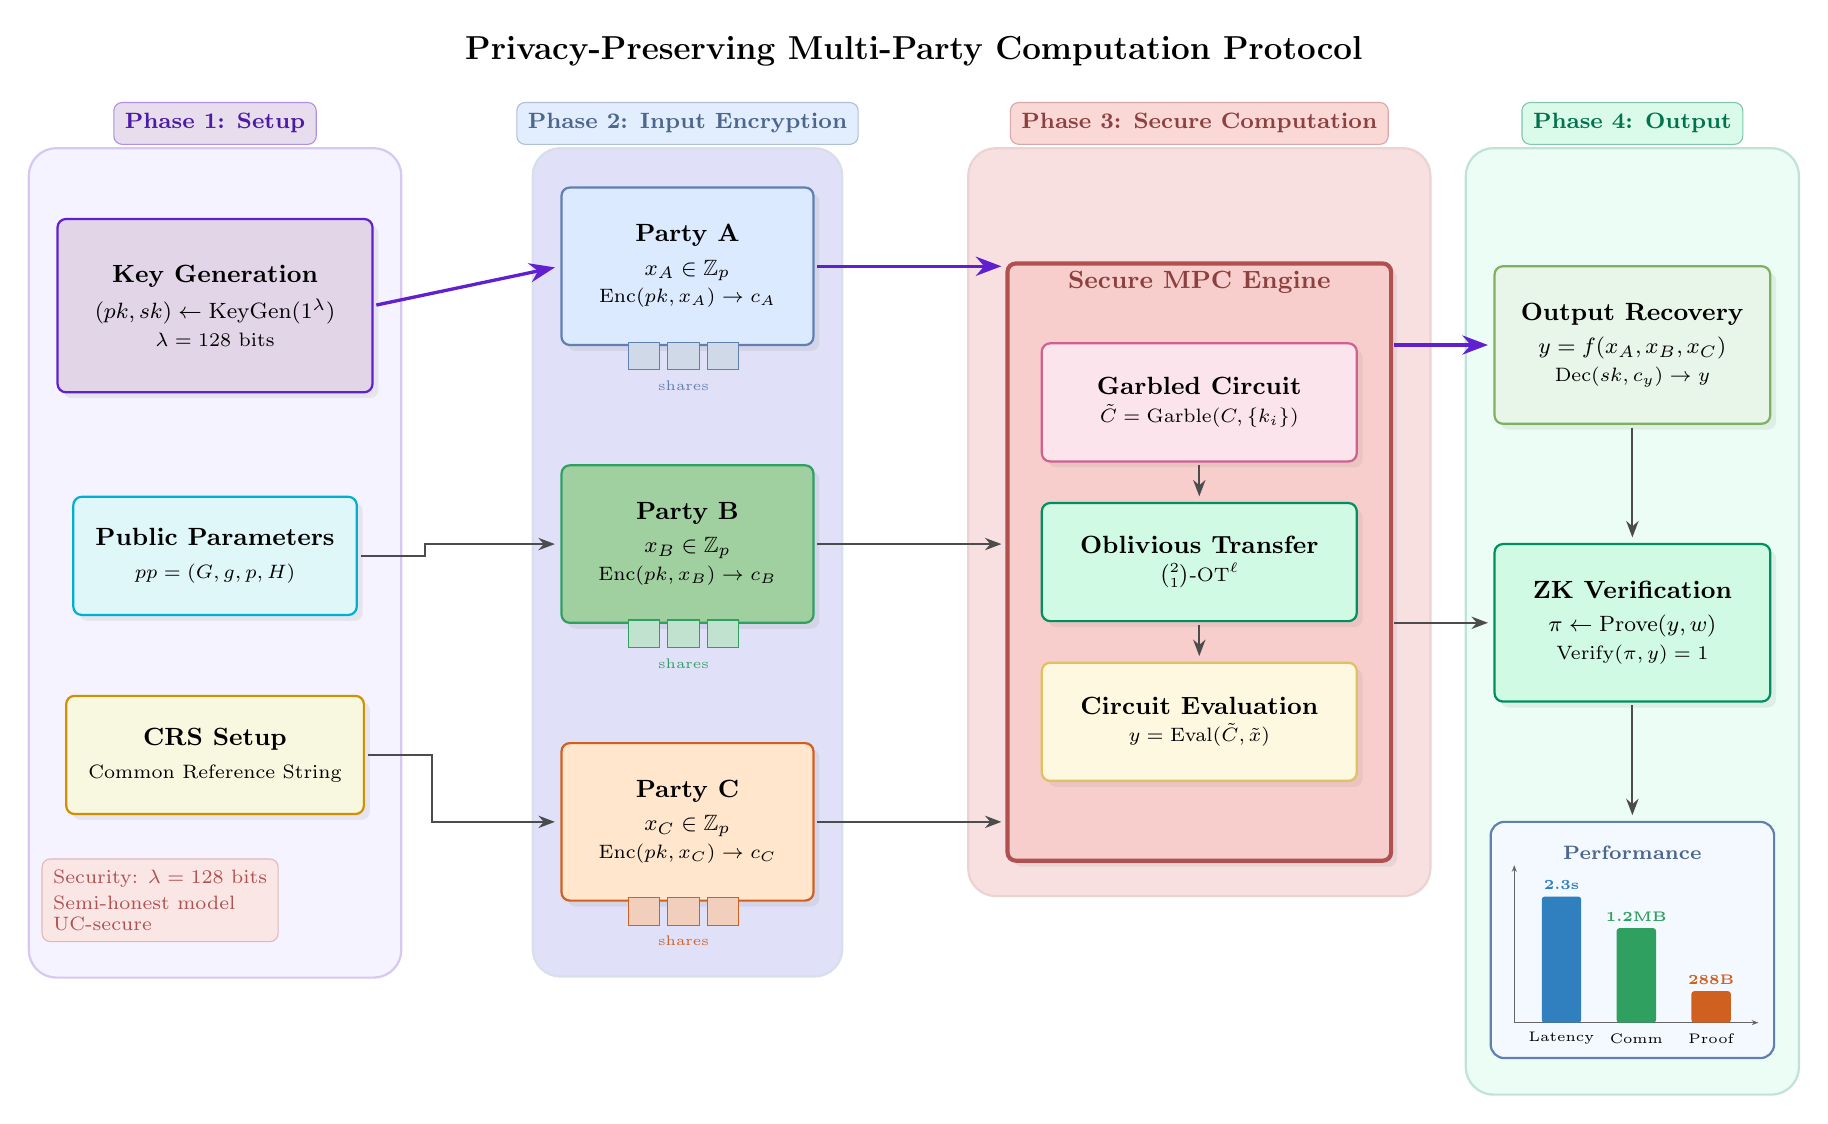
\begin{tikzpicture}[
    every node/.style={font=\small},
    base_box/.style={rectangle, rounded corners=3pt, align=center,
        minimum height=0.9cm, minimum width=2.6cm,
        inner sep=8pt, drop shadow={opacity=0.12}, thick},
    blue_node/.style={base_box, fill=acaBlueFill, draw=acaBlueLine},
    green_node/.style={base_box, fill=acaGreenFill, draw=acaGreenLine},
    orange_node/.style={base_box, fill=acaOrangeFill, draw=acaOrangeLine},
    purple_node/.style={base_box, fill=acaPurpleFill, draw=acaPurpleLine},
    red_node/.style={base_box, fill=acaRedFill, draw=acaRedLine, font=\small\bfseries},
    grey_node/.style={base_box, fill=acaGreyFill, draw=acaGreyLine},
    gold_node/.style={base_box, fill=acaGoldFill, draw=acaGoldLine},
    teal_node/.style={base_box, fill=acaTealFill, draw=acaTealLine},
    cyan_node/.style={base_box, fill=acaCyanFill, draw=acaCyanLine},
    pink_node/.style={base_box, fill=acaPinkFill, draw=acaPinkLine},
    yellow_node/.style={base_box, fill=acaYellowFill, draw=acaYellowLine},
    lime_node/.style={base_box, fill=acaLimeFill, draw=acaLimeLine},
    arrow/.style={-{Stealth[scale=0.9]}, thick, color=black!70, shorten >=2pt, shorten <=1pt},
    data_arrow/.style={-{Stealth[scale=1.1]}, very thick, color=acaPurpleLine, shorten >=2pt, shorten <=1pt},
]

% ================================================================
%  COLUMN REFERENCE CENTERS — spaced left->right by \colgap.
%  Re-spacing the whole figure = change \colgap in one place.
% ================================================================
\coordinate (c1) at (2.5, 0);
\coordinate (c2) at ($(c1)+(\gapAB,0)$);
\coordinate (c3) at ($(c2)+(\gapBC,0)$);
\coordinate (c4) at ($(c3)+(\gapCD,0)$);

% ================================================================
%  Phase 1: Key Generation — column on (c1), top-anchored chain
% ================================================================
\node[purple_node, minimum width=4cm, minimum height=2.2cm]
    (keygen) at (c1 |- 0,14.5)
    {\textbf{Key Generation}\\[2pt]{\footnotesize $(pk, sk) \leftarrow \mathrm{KeyGen}(1^\lambda)$}\\[-1pt]{\scriptsize $\lambda = 128$ bits}};

\node[cyan_node, minimum width=3.5cm, minimum height=1.5cm, below=1.3cm of keygen]
    (params)
    {\textbf{Public Parameters}\\[1pt]{\scriptsize $pp = (G, g, p, H)$}};

\node[gold_node, minimum width=3.5cm, minimum height=1.5cm, below=1.0cm of params]
    (crs)
    {\textbf{CRS Setup}\\[1pt]{\scriptsize Common Reference String}};

% Security annotation — part of Phase 1 column; placed before the zone fit
% so the zone background grows to contain it (no hand-typed bottom y).
\node[font=\scriptsize, text=acaRedLine, fill=acaRedFill!50, draw=acaRedLine!40,
      rounded corners=3pt, inner sep=4pt, anchor=north west]
      at ($(crs.south west)+(-0.3,-0.55)$) (secnote)
    {\shortstack[l]{Security: $\lambda = 128$ bits\\Semi-honest model\\UC-secure}};

% ================================================================
%  Phase 2: Encryption & Secret Sharing — column on (c2)
% ================================================================
% Party A
\node[blue_node, minimum width=3.2cm, minimum height=2.0cm]
    (partyA) at (c2 |- 0,15.0)
    {\textbf{Party A}\\[1pt]{\footnotesize $x_A \in \mathbb{Z}_p$}\\[-1pt]{\scriptsize Enc$(pk, x_A) \to c_A$}};
% Party B
\node[green_node, minimum width=3.2cm, minimum height=2.0cm, below=1.5cm of partyA]
    (partyB)
    {\textbf{Party B}\\[1pt]{\footnotesize $x_B \in \mathbb{Z}_p$}\\[-1pt]{\scriptsize Enc$(pk, x_B) \to c_B$}};
% Party C
\node[orange_node, minimum width=3.2cm, minimum height=2.0cm, below=1.5cm of partyB]
    (partyC)
    {\textbf{Party C}\\[1pt]{\footnotesize $x_C \in \mathbb{Z}_p$}\\[-1pt]{\scriptsize Enc$(pk, x_C) \to c_C$}};

% Secret sharing visualization — small matrix BELOW each party box.
% Re-anchored to the party node: scope shifted to each party's .south, so
% the shares row travels with its party box under any reflow.
\foreach \party/\col in {partyA/acaBlueLine, partyB/acaGreenLine, partyC/acaOrangeLine} {
  \begin{scope}[shift={($(\party.south)+(0,-0.30)$)}]
    \foreach \s in {0,1,2} {
      \fill[\col!30] ({(\s-1.5)*0.5}, 0) rectangle ({(\s-1.5)*0.5+0.4}, 0.35);
      \draw[\col, thin] ({(\s-1.5)*0.5}, 0) rectangle ({(\s-1.5)*0.5+0.4}, 0.35);
    }
    \node[font=\tiny, text=\col] at (-0.05, -0.2) {shares};
  \end{scope}
}

% ================================================================
%  Phase 3: Secure Computation — Core engine on (c3)
% ================================================================
% Engine border FIRST (empty bordered box, fitted around its sub-modules).
% We pre-declare the sub-box positions via coordinates, build the border,
% then draw the sub-boxes on top so they remain visible.
\node[font=\small\bfseries, text=acaRedLine!80!black]
    (mpclabel) at (c3 |- 0,14.8) {Secure MPC Engine};

\node[pink_node, minimum width=4.0cm, minimum height=1.5cm, below=0.5cm of mpclabel]
    (garbled)
    {\textbf{Garbled Circuit}\\[-1pt]{\scriptsize $\tilde{C} = \mathrm{Garble}(C, \{k_i\})$}};
\node[teal_node, minimum width=4.0cm, minimum height=1.5cm, below=0.5cm of garbled]
    (ot)
    {\textbf{Oblivious Transfer}\\[-1pt]{\scriptsize $\binom{2}{1}\text{-OT}^\ell$}};
\node[yellow_node, minimum width=4.0cm, minimum height=1.5cm, below=0.5cm of ot]
    (eval)
    {\textbf{Circuit Evaluation}\\[-1pt]{\scriptsize $y = \mathrm{Eval}(\tilde{C}, \tilde{x})$}};

% Engine extent rails — invisible coordinates that give the engine box the
% original's generous ~1cm of internal padding above the top sub-box and
% below the bottom sub-box (the original used a fixed 7.5cm-tall box). The
% engine fit spans these so its proportions match without hand-sizing.
\coordinate (engtop) at ($(garbled.north)+(0,1.0)$);
\coordinate (engbot) at ($(eval.south)+(0,-1.0)$);

% Engine anchor — an INVISIBLE fit node spanning the rails + sub-modules.
% It only provides the (mpc) anchors used by the cross-phase arrows; the
% VISIBLE engine box (red fill + thick border) is drawn later, in the
% background layer AFTER the zone fills, so it paints on top of the zone
% but stays behind the sub-boxes. Replaces the hand-sized 5.5x7.5cm box.
\node[fit=(engtop)(engbot)(garbled)(ot)(eval), draw=none, fill=none,
      inner xsep=12pt, inner ysep=0pt] (mpc) {};

% Internal arrows — node anchors only.
\draw[arrow] (garbled.south) -- (ot.north);
\draw[arrow] (ot.south) -- (eval.north);

% ================================================================
%  Phase 4: Output & Verification — column on (c4)
% ================================================================
\node[lime_node, minimum width=3.5cm, minimum height=2.0cm]
    (output) at (c4 |- 0,14.0)
    {\textbf{Output Recovery}\\[1pt]{\footnotesize $y = f(x_A, x_B, x_C)$}\\[-1pt]{\scriptsize Dec$(sk, c_y) \to y$}};

\node[teal_node, minimum width=3.5cm, minimum height=2.0cm, below=1.5cm of output]
    (verify)
    {\textbf{ZK Verification}\\[1pt]{\footnotesize $\pi \leftarrow \mathrm{Prove}(y, w)$}\\[-1pt]{\scriptsize $\mathrm{Verify}(\pi, y) = 1$}};

% Performance panel — width 3.6cm (leaves margin inside the Phase 4 zone).
\node[rectangle, rounded corners=5pt, draw=acaBlueLine, fill=acaBlueFill!30,
      minimum width=3.6cm, minimum height=3.0cm, thick, below=1.5cm of verify]
      (perf) {};
\node[font=\scriptsize\bfseries, text=acaBlueLine!80!black, anchor=north]
      at ($(perf.north)+(0,-0.2)$) {Performance};

% Mini bar chart — kept intact, re-anchored to the perf node centre.
% Local origin at the axis foot; everything in perf-local coords.
\begin{scope}[shift={($(perf.center)+(-1.7,-1.05)$)}]
  \draw[-{Stealth[scale=0.5]}, acaGreyLine] (0.2, 0) -- (0.2, 2.0);
  \draw[-{Stealth[scale=0.5]}, acaGreyLine] (0.2, 0) -- (3.3, 0);
  \fill[barBlue, rounded corners=1pt] (0.55, 0) rectangle (1.05, 1.6);
  \fill[barGreen, rounded corners=1pt] (1.50, 0) rectangle (2.00, 1.2);
  \fill[barOrange, rounded corners=1pt] (2.45, 0) rectangle (2.95, 0.4);
  \node[font=\tiny] at (0.8, -0.2) {Latency};
  \node[font=\tiny] at (1.75, -0.2) {Comm};
  \node[font=\tiny] at (2.7, -0.2) {Proof};
  \node[font=\tiny\bfseries, text=barBlue] at (0.8, 1.75) {2.3s};
  \node[font=\tiny\bfseries, text=barGreen] at (1.75, 1.35) {1.2MB};
  \node[font=\tiny\bfseries, text=barOrange] at (2.7, 0.55) {288B};
\end{scope}

% ================================================================
%  ZONE BACKGROUNDS — built with `fit` over each column's contents +
%  a per-zone UNIFORM-top rail coordinate (all share y=\ztop) so every
%  zone top aligns. Bottoms grow to each column's lowest element.
%  The rail coordinates carry no visible mark; they only pin the fit.
% ================================================================
% Per-column top-rail coordinates at the shared \ztop level.
\coordinate (t1) at (c1 |- 0,\ztop);
\coordinate (t2) at (c2 |- 0,\ztop);
\coordinate (t3) at (c3 |- 0,\ztop);
\coordinate (t4) at (c4 |- 0,\ztop);

% Per-zone bottom rails — pin each zone's lower edge a uniform ~0.45cm
% below its lowest content, so all four zones share the same bottom margin
% (matching the original's deliberate breathing room under each column).
\def\zbotpad{0.45}
\coordinate (b1) at ($(secnote.south)+(0,-\zbotpad)$);
\coordinate (b2) at ($(partyC.south)+(0,-0.95)$);   % below partyC shares row
\coordinate (b3) at ($(engbot)+(0,-\zbotpad)$);     % below the engine box
\coordinate (b4) at ($(perf.south)+(0,-\zbotpad)$);

\begin{pgfonlayer}{background}
  % Phase 1 zone — fit over keygen..secnote + top rail + bottom rail.
  \node[fit=(t1)(keygen)(b1), inner xsep=10pt, inner ysep=0pt,
        rounded corners=10pt, fill=zonePurpleBg, draw=acaPurpleLine!25,
        thick] (zone1) {};
  % Phase 2 zone — fit over party column + top rail + bottom shares rail.
  \node[fit=(t2)(partyA)(b2), inner xsep=10pt, inner ysep=0pt,
        rounded corners=10pt, fill=zoneBlueBg, draw=acaBlueLine!25,
        thick] (zone2) {};
  % Phase 3 zone — fit over the (invisible) MPC engine box + top/bottom rail,
  % with extra x-padding so the visible engine border keeps a side margin.
  \node[fit=(t3)(mpc)(b3), inner xsep=14pt, inner ysep=0pt,
        rounded corners=10pt, fill=zoneRedBg, draw=acaRedLine!25,
        thick] (zone3) {};
  % Phase 4 zone — fit over output..perf + top rail + bottom rail.
  \node[fit=(t4)(output)(b4), inner xsep=10pt, inner ysep=0pt,
        rounded corners=10pt, fill=zoneGreenBg, draw=acaTealLine!25,
        thick] (zone4) {};
\end{pgfonlayer}

% Visible MPC engine box — drawn in the background layer AFTER the zone
% fills, so the red fill + thick border sit ON TOP of the zone3 fill but
% BEHIND the (main-layer) sub-boxes. fit over the same content as the
% invisible (mpc) anchor so the two coincide exactly.
\begin{pgfonlayer}{background}
  \node[red_node, fit=(engtop)(engbot)(garbled)(ot)(eval),
        inner xsep=12pt, inner ysep=0pt, line width=1.5pt] (mpcbox) {};
\end{pgfonlayer}

% ================================================================
%  CONNECTIONS — all via NODE ANCHORS
% ================================================================
% Phase 1 → Phase 2
\draw[data_arrow] (keygen.east) -- (partyA.west);
\draw[arrow] (params.east) -- ++(0.85, 0) |- (partyB.west);
\draw[arrow] (crs.east) -- ++(0.85, 0) |- (partyC.west);

% Phase 2 → Phase 3
\draw[data_arrow, rounded corners=6pt] (partyA.east) -- (mpc.west |- partyA);
\draw[arrow, rounded corners=6pt] (partyB.east) -- (mpc.west |- partyB);
\draw[arrow, rounded corners=6pt] (partyC.east) -- (mpc.west |- partyC);

% Phase 3 → Phase 4
\draw[data_arrow, rounded corners=6pt] (mpc.east |- output) -- (output.west);
\draw[arrow, rounded corners=6pt] (mpc.east |- verify) -- (verify.west);

% Output → Verify
\draw[arrow] (output.south) -- (verify.north);

% Verify → Performance
\draw[arrow] (verify.south) -- (perf.north);

% ================================================================
%  PHASE LABELS — chips anchored UNIFORMLY to each zone .north (gap 0.3cm)
% ================================================================
\node[font=\footnotesize\bfseries, fill=acaPurpleFill!80, draw=acaPurpleLine!50,
      rounded corners=3pt, inner sep=4pt, text=acaPurpleLine!80!black, anchor=center]
      at ($(zone1.north)+(0,0.3)$) {Phase 1: Setup};
\node[font=\footnotesize\bfseries, fill=acaBlueFill!80, draw=acaBlueLine!50,
      rounded corners=3pt, inner sep=4pt, text=acaBlueLine!80!black, anchor=center]
      at ($(zone2.north)+(0,0.3)$) {Phase 2: Input Encryption};
\node[font=\footnotesize\bfseries, fill=acaRedFill!80, draw=acaRedLine!50,
      rounded corners=3pt, inner sep=4pt, text=acaRedLine!80!black, anchor=center]
      at ($(zone3.north)+(0,0.3)$) {Phase 3: Secure Computation};
\node[font=\footnotesize\bfseries, fill=acaTealFill!80, draw=acaTealLine!50,
      rounded corners=3pt, inner sep=4pt, text=acaTealLine!80!black, anchor=center]
      at ($(zone4.north)+(0,0.3)$) {Phase 4: Output};

% ================================================================
%  Title — centred via calc midpoint of the whole zone row
% ================================================================
\coordinate (rowtop) at ($(zone1.north west)!0.5!(zone4.north east)$);
\node[font=\large\bfseries, anchor=south] at ($(rowtop)+(0,0.9)$)
    {Privacy-Preserving Multi-Party Computation Protocol};

\end{tikzpicture}
\end{document}
